\documentclass[a4paper,12pt]{article}
\usepackage[paper=a4paper,left=35mm,right=25mm,top=25mm,bottom=20mm]{geometry}
\usepackage[ngerman]{babel}
\usepackage[utf8]{inputenc}
\usepackage{amsmath}
\usepackage{amssymb}
\usepackage{tikz}
\usepackage{enumitem}
\usepackage{cite}
\usepackage{natbib}
\usepackage{graphicx}
\usepackage{float}

\linespread{1.5}

\addto\captionsngerman{
  \renewcommand{\contentsname}
    {INHALTSVERZEICHNIS}
}


\begin{document}
\parindent0cm

%===================================================================================
%---------------------------- TITELSEITE -------------------------------------------
%===================================================================================

\thispagestyle{empty}

\begin{center}

\begin{large} 
GYMNASIUM OTTOBRUNN	\\
\vspace{1cm}
Oberstufenjahrgang 2017/19\\
\vspace{1cm}
Seminarfach Softwareentwicklung\\
\vspace{2cm}
Seminararbeit\\
\end{large}


\vspace{1cm}


{\Huge\bfseries 
36. Bundeswettbewerb Informatik\par
Runde 2\par
Aufgabe 1 und 3\par 
}


\vspace{2cm}


\begin{large}
\begin{tabular}{rl}
Verfasser:& Jonas Fritsch \\
Seminarleiter: & StD Peter Brichzin \\
Bewertung:  & ......... Punkte  \\
Unterschrift des Seminarleiters: & ...........................................  \\
\end{tabular} 
\end{large}

\end{center}

%===================================================================================
%---------------------------- INHALTSVERZEICHNIS -----------------------------------
%===================================================================================				

\newpage

\thispagestyle{empty}
\tableofcontents	


\setcounter{page}{2}

%===================================================================================
%-------------------------------- EINLEITUNG ---------------------------------------
%===================================================================================

\newpage
\section{EINLEITUNG}



Lorem ipsum dolor sit amet, consectetur adipiscing elit. Sed tempus consectetur lorem, imperdiet dignissim est auctor a. Vivamus convallis, leo et iaculis egestas, nunc massa porttitor tellus, id faucibus urna justo eget massa. Praesent quis feugiat odio. Nullam quis mattis enim. Fusce volutpat odio in enim sodales venenatis. Mauris consequat.

%===================================================================================
%-------------------------------- AUFGABE 1 ----------------------------------------
%===================================================================================

\newpage
\section{AUFGABE 1 - "Die Kunst der Fuge"}



\subsection{Aufgabenstellung}
Ilona besitzt einen riesigen Haufen Holzklötzchen: Diese haben alle dieselbe Höhe und Tiefe,
aber verschiedene Längen. \\
Ilona möchte eine Mauer bauen. Jede Reihe der Mauer soll aus $n$ Klötzchen bestehen, die die
Längen 1 bis $n$ haben und lückenlos aneinander liegen. Die Stellen zwischen den Klötzchen heißen
Fugen. Ilona möchte, dass in der fertigen Mauer niemals zwei Fugen übereinander liegen,
selbst wenn sich mehrere Reihen dazwischen befinden. Außerdem soll ihre Mauer möglichst
hoch sein. \\
Für $n = 4$ gelingt es ihr recht schnell, eine Mauer mit drei Reihen zu bauen:
\begin{figure}[H]
    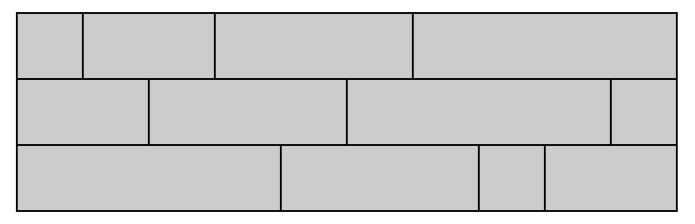
\includegraphics[width=0.7\linewidth]{Bilder/Aufgabe1/Aufgabenstellung_BeispielMauer.png}
\end{figure}
\begin{large}
    \textbf{Aufgabe} \\
\end{large}
Hilf Ilona, indem du ein Programm schreibst, das nach Eingabe von $n$ eine nach ihren Vorgaben
konstruierte, möglichst hohe Mauer ausgibt. Für $n = 10$ sollte dein Programm eine Mauer der
Höhe 6 ausgeben können. Wie hoch werden die Mauern deines Programms für größere $n$?

\subsection{Lösungsidee}

\subsection{Implementierung}

\subsection{Laufzeitanalyse}

\subsection{Optimierungsmöglichkeiten}

\subsection{Beispiele}

\subsection{Quellcode}

%===================================================================================
%-------------------------------- AUFGABE 3 ----------------------------------------
%===================================================================================

\newpage
\section{AUFGABE 3 - "Quo vadis, Quax?"}



\subsection{Aufgabenstellung}

\subsection{Lösungsidee}

\subsection{Teilaufgabe (a)}

\subsection{Teilaufgabe (b)}

\subsection{Teilaufgabe (c)}
\subsubsection{Implementierung}
\subsubsection{Laufzeitanalyse}
\subsubsection{Optimierungsmöglichkeiten}
\subsubsection{Beispiele}

\subsection{Teilaufgabe (d)}

\subsection{Quellcode}

%===================================================================================
%---------------------------------- FAZIT ------------------------------------------
%===================================================================================

\newpage
\section{FAZIT}



Lorem ipsum dolor sit amet, consectetur adipiscing elit. Sed tempus consectetur lorem, imperdiet dignissim est auctor a. Vivamus convallis, leo et iaculis egestas, nunc massa porttitor tellus, id faucibus urna justo eget massa. Praesent quis feugiat odio. Nullam quis mattis enim. Fusce volutpat odio in enim sodales venenatis. Mauris consequat.

%===================================================================================
%--------------------------- ABBILDUNGSVERZEICHNIS ---------------------------------
%===================================================================================

\newpage
\section{ABBILDUNGSVERZEICHNIS}



Lorem ipsum dolor sit amet, consectetur adipiscing elit. Sed tempus consectetur lorem, imperdiet dignissim est auctor a. Vivamus convallis, leo et iaculis egestas, nunc massa porttitor tellus, id faucibus urna justo eget massa. Praesent quis feugiat odio. Nullam quis mattis enim. Fusce volutpat odio in enim sodales venenatis. Mauris consequat.

%===================================================================================
%--------------------------- LITERATURVERZEICHNIS ----------------------------------
%===================================================================================

\newpage
\section{LITERATURVERZEICHNIS}



Lorem ipsum dolor sit amet, consectetur adipiscing elit. Sed tempus consectetur lorem, imperdiet dignissim est auctor a. Vivamus convallis, leo et iaculis egestas, nunc massa porttitor tellus, id faucibus urna justo eget massa. Praesent quis feugiat odio. Nullam quis mattis enim. Fusce volutpat odio in enim sodales venenatis. Mauris consequat.

%===================================================================================
%------------------------- ERKLÄRUNG DES VERFASSERS --------------------------------
%===================================================================================

\newpage
\section{ERKLÄRUNG DES VERFASSERS}



Lorem ipsum dolor sit amet, consectetur adipiscing elit. Sed tempus consectetur lorem, imperdiet dignissim est auctor a. Vivamus convallis, leo et iaculis egestas, nunc massa porttitor tellus, id faucibus urna justo eget massa. Praesent quis feugiat odio. Nullam quis mattis enim. Fusce volutpat odio in enim sodales venenatis. Mauris consequat.

\begin{figure}[H]
    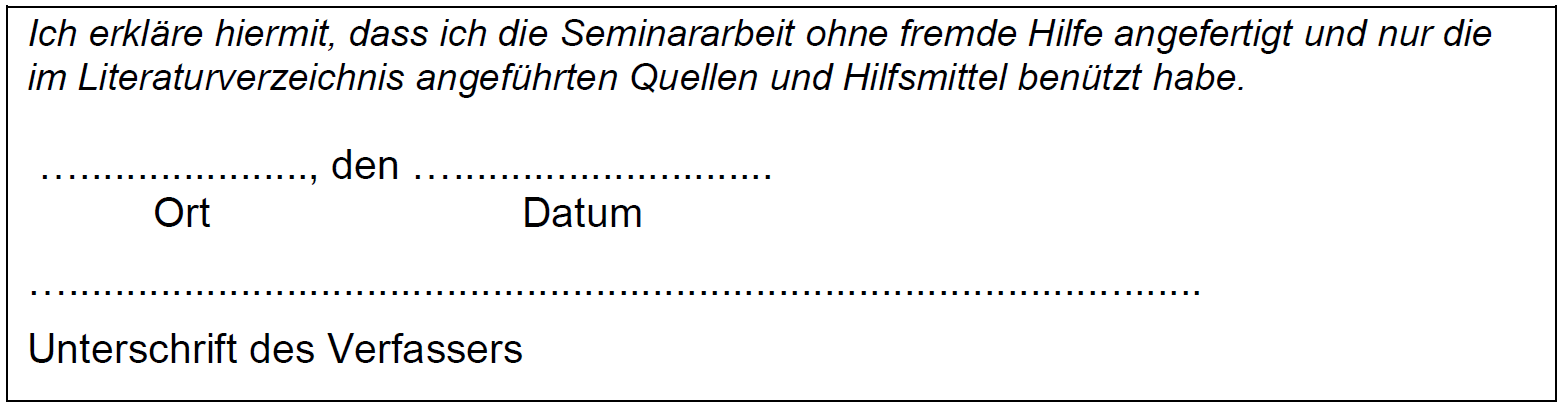
\includegraphics[width=\linewidth]{Bilder/Sonstiges/ErklaerungDesVerfassers.png}
\end{figure}

\end{document}